\documentclass[aspectratio=169,professionalfonts]{beamer}

% ----- THEME AND PACKAGES -----
\usetheme{UGM}
\usefonttheme{professionalfonts}
\usepackage[type1, sfdefault]{atkinson}
\usepackage[T1]{fontenc}
\usepackage{booktabs}
\usepackage{multicol}
\usepackage{graphicx}

% ----- PRESENTATION METADATA -----
\title{Skin Lesion Classification for\\Monkeypox Detection}
\subtitle{Hybrid Handcrafted and CNN Feature Approach}
\author{Yusuf Imantaka Bastari \and Aufa Sultan Syach Majid Putra Yuliyanto}
\institute{Department of Computer Science and Electronics\\Universitas Gadjah Mada\\Yogyakarta, Indonesia}
\date{June 2, 2026}

\begin{document}

% ----- TITLE FRAME -----
\begin{frame}[plain]
    \titlepage
\end{frame}

% ----- OUTLINE -----
\begin{frame}
    \frametitle{Outline}
    \begin{multicols}{2}
        \tableofcontents
    \end{multicols}
\end{frame}

% ----- SECTION: INTRODUCTION -----
\section{Introduction}

\begin{frame}
    \frametitle{Background}
    \footnotesize
    
    \begin{columns}[T]
        \begin{column}{0.52\textwidth}
            \textbf{Monkeypox (MPX)} is a zoonotic disease caused by the Monkeypox virus.
            \begin{itemize}
                \footnotesize
                \setlength{\itemsep}{2pt}
                \item Endemic to Central and West Africa
                \item 2022--2023 global outbreak highlighted urgent need for rapid diagnostics
                \item Visual inspection is the primary diagnostic method
                \item Easily confused with chickenpox, measles, and other rashes
            \end{itemize}
            \vspace{0.3em}
            \alert{Challenge:} Automated classification needed for timely diagnosis.
        \end{column}
        
        \begin{column}{0.42\textwidth}
            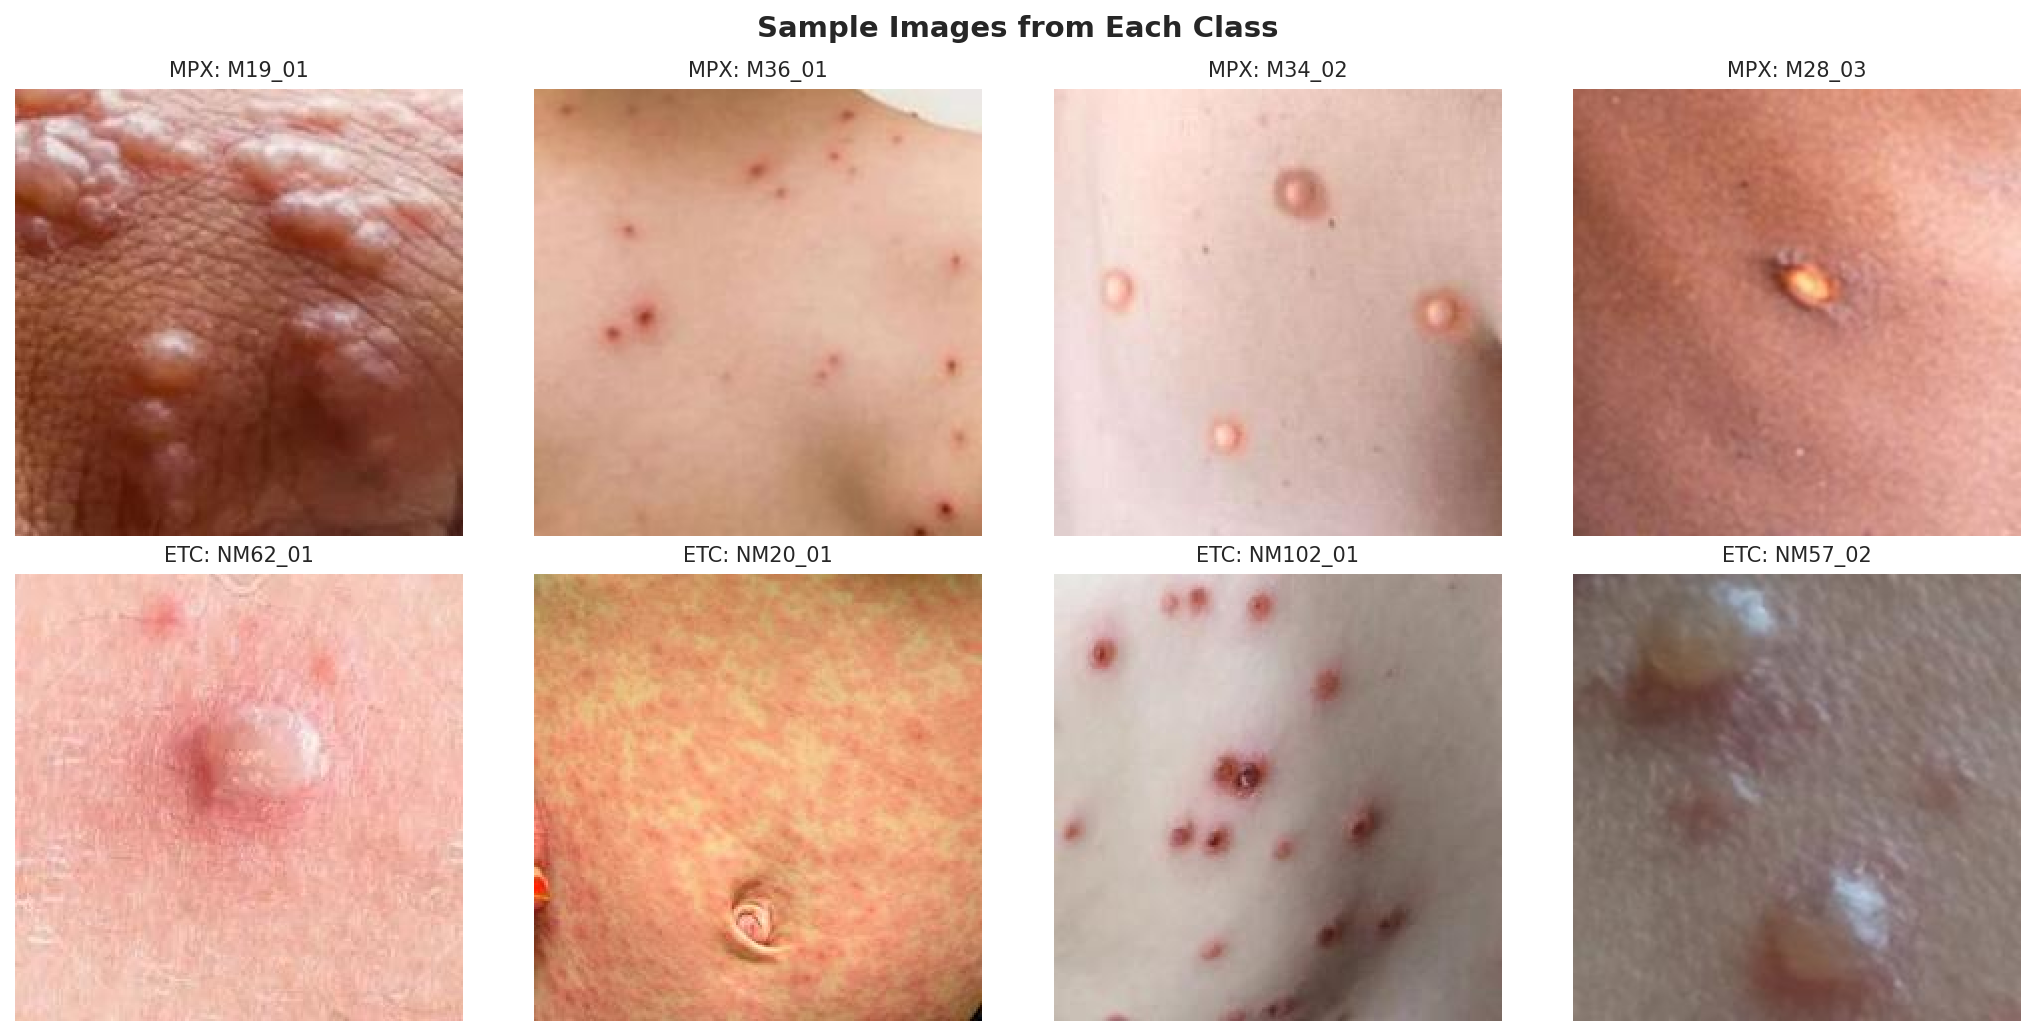
\includegraphics[width=\textwidth]{sample_images.png}
            \centerline{\footnotesize Sample skin lesion images}
        \end{column}
    \end{columns}
\end{frame}

\begin{frame}
    \frametitle{Problem Statement \& Objectives}
    \footnotesize
    
    \begin{block}{\footnotesize Problem Statement}
        \footnotesize
        Skin lesions from Monkeypox are visually similar to other conditions, making manual diagnosis error-prone and time-consuming.
    \end{block}
    
    \vspace{0.3em}
    
    \begin{exampleblock}{\footnotesize Research Objectives}
        \footnotesize
        \begin{enumerate}
            \setlength{\itemsep}{1pt}
            \item Robust lesion segmentation from skin background
            \item Handcrafted features (color, texture, shape, edges, frequency)
            \item Transfer-learned CNN embeddings (ResNet18)
            \item Compare handcrafted, CNN, and hybrid representations
            \item Evaluate classifiers for binary MPX vs. non-MPX
        \end{enumerate}
    \end{exampleblock}
\end{frame}

% ----- SECTION: DATASET -----
\section{Dataset \& Preprocessing}

\begin{frame}
    \frametitle{Dataset Description}
    \footnotesize
    
    \begin{columns}[T]
        \begin{column}{0.48\textwidth}
            \textbf{Source:} Monkeypox Skin Lesion Dataset (Kaggle)
            \begin{itemize}
                \footnotesize
                \setlength{\itemsep}{2pt}
                \item 228 skin lesion images (224$\times$224 RGB)
                \item \textbf{MPX:} 102 images (45\%)
                \item \textbf{Non-MPX:} 126 images (55\%)
            \end{itemize}
            \vspace{0.3em}
            \textbf{Split:} Stratified 70/30
            \begin{itemize}
                \footnotesize
                \setlength{\itemsep}{2pt}
                \item Training: 160 images
                \item Testing: 68 images
            \end{itemize}
        \end{column}
        
        \begin{column}{0.45\textwidth}
            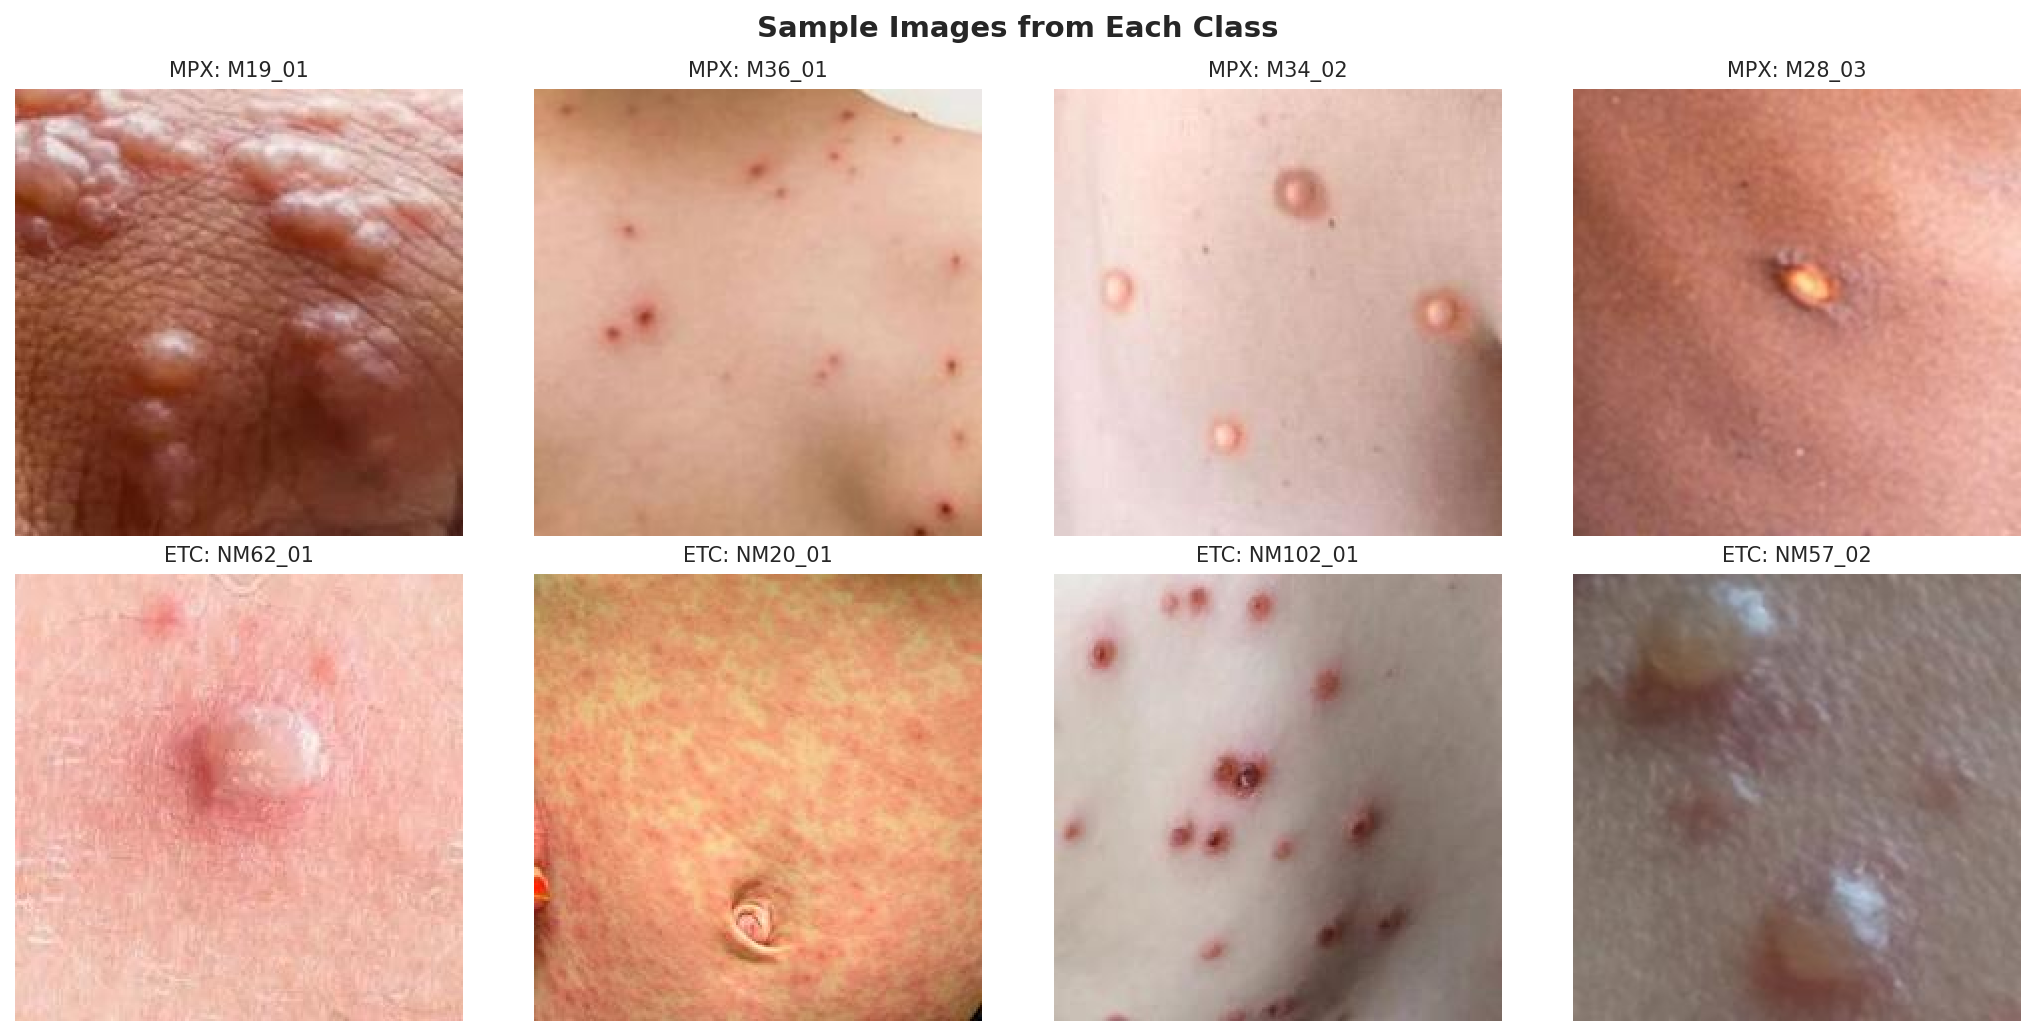
\includegraphics[width=\textwidth]{sample_images.png}
            \centerline{\footnotesize Dataset sample images}
        \end{column}
    \end{columns}
\end{frame}

\begin{frame}
    \frametitle{Lesion Segmentation Pipeline}
    \footnotesize
    
    \begin{columns}[T]
        \begin{column}{0.42\textwidth}
            \textbf{Method:} LAB + CLAHE + Otsu + Morphology
            \vspace{0.2em}
            \begin{enumerate}
                \footnotesize
                \setlength{\itemsep}{1pt}
                \item BGR $\rightarrow$ LAB conversion
                \item CLAHE on $L^*$ and $a^*$ channels
                \item Combine $L^*$ + inverted $a^*$ (0.3, 0.7)
                \item Otsu thresholding
                \item Morphological closing + opening
                \item Keep largest connected component
            \end{enumerate}
            \vspace{0.2em}
            \alert{Result:} Clean binary mask isolating the lesion.
        \end{column}
        
        \begin{column}{0.52\textwidth}
            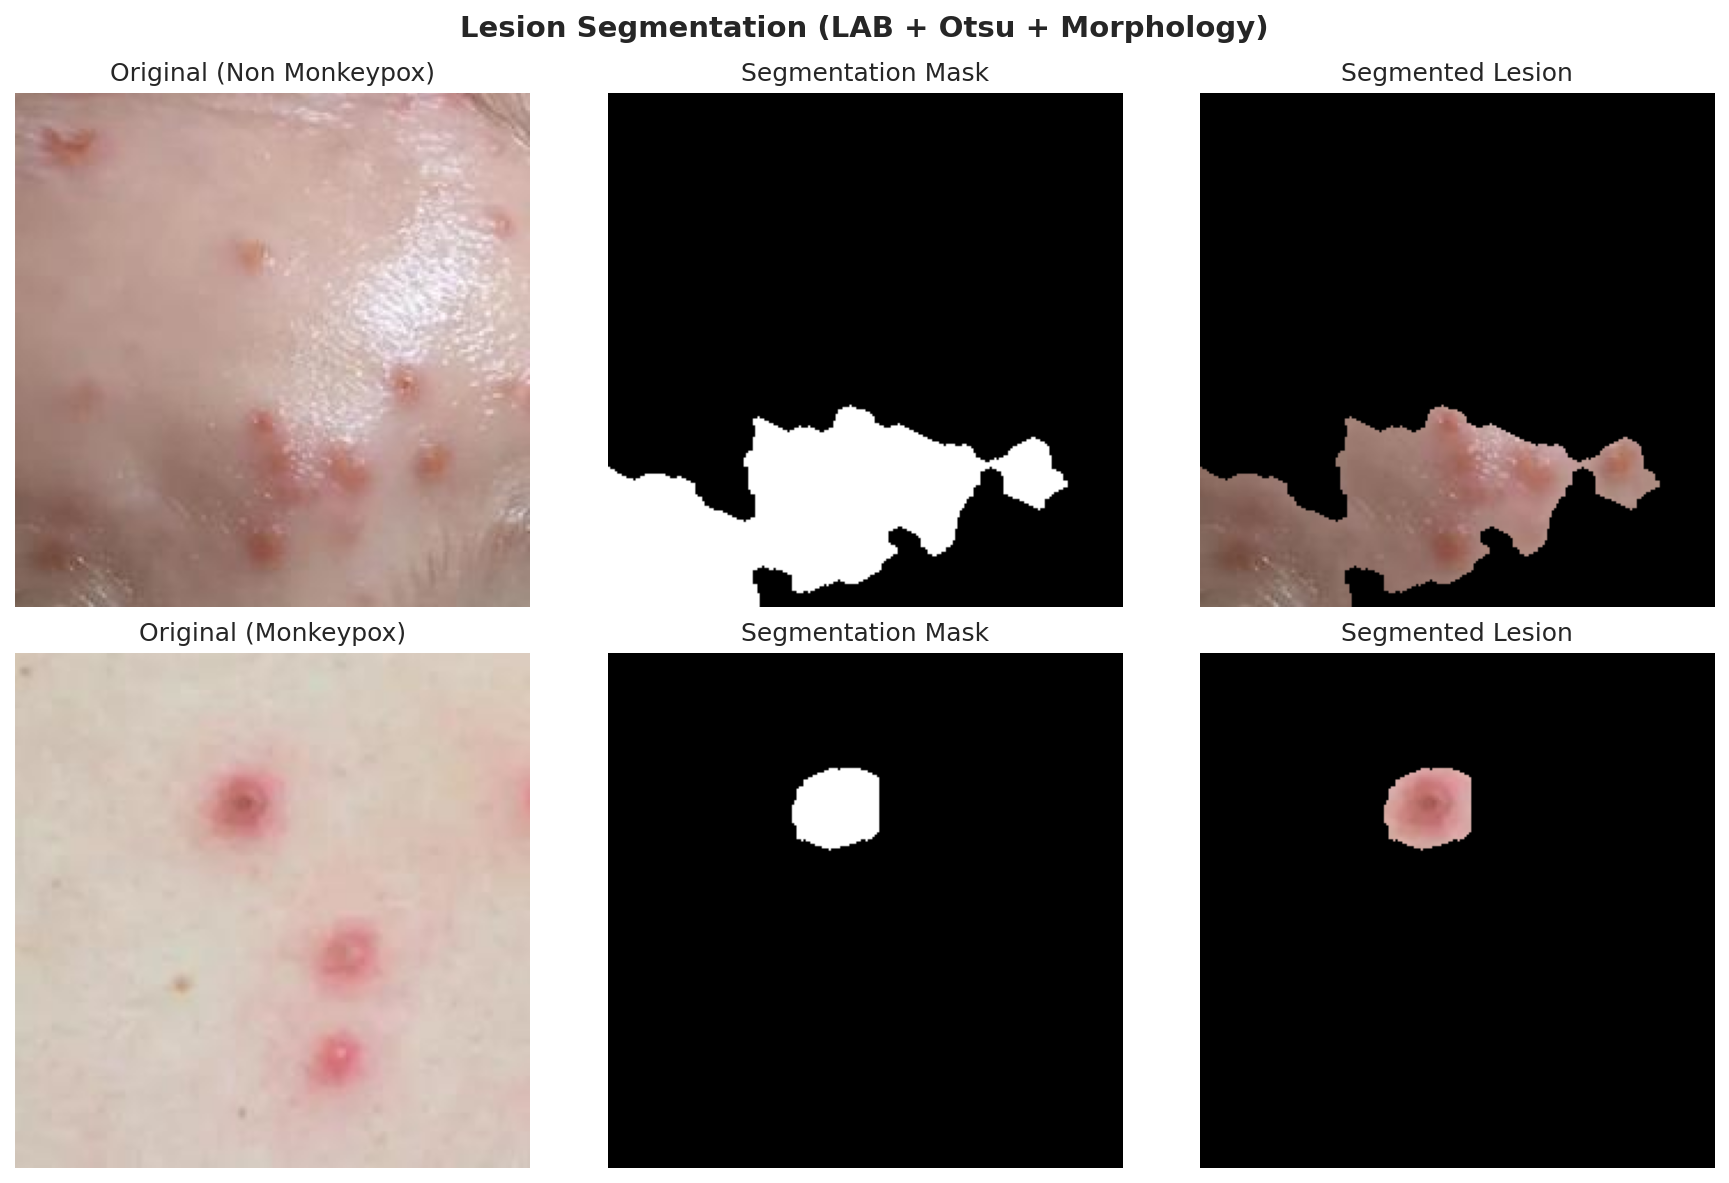
\includegraphics[width=\textwidth]{segmentation_example.png}
            \centerline{\footnotesize Segmentation results}
        \end{column}
    \end{columns}
\end{frame}

% ----- SECTION: METHODOLOGY -----
\section{Methodology}

\begin{frame}
    \frametitle{Handcrafted Feature Extraction}
    \footnotesize
    
    \begin{columns}[T]
        \begin{column}{0.48\textwidth}
            \textbf{Seven categories, $\sim$200 raw features}
            \vspace{0.2em}
            \begin{itemize}
                \footnotesize
                \setlength{\itemsep}{1pt}
                \item \textbf{Color} (84): Moments, HSV hist., percentiles in BGR/HSV/LAB
                \item \textbf{GLCM} (10): Contrast, dissimilarity, homogeneity, energy, correlation
                \item \textbf{LBP} (18): Uniform patterns, $r$=2, $P$=16
                \item \textbf{Gabor} (12): 3 orientations $\times$ 2 scales
                \item \textbf{Shape} (12): Hu moments + geometric properties
                \item \textbf{Edge} (3): Canny density + Sobel gradient
                \item \textbf{FFT} (16): Radial power spectrum rings
            \end{itemize}
            \vspace{0.2em}
            After variance filtering: \alert{155 features}
        \end{column}
        
        \begin{column}{0.48\textwidth}
            \textbf{Feature importance (by category)}
            \vspace{0.2em}
            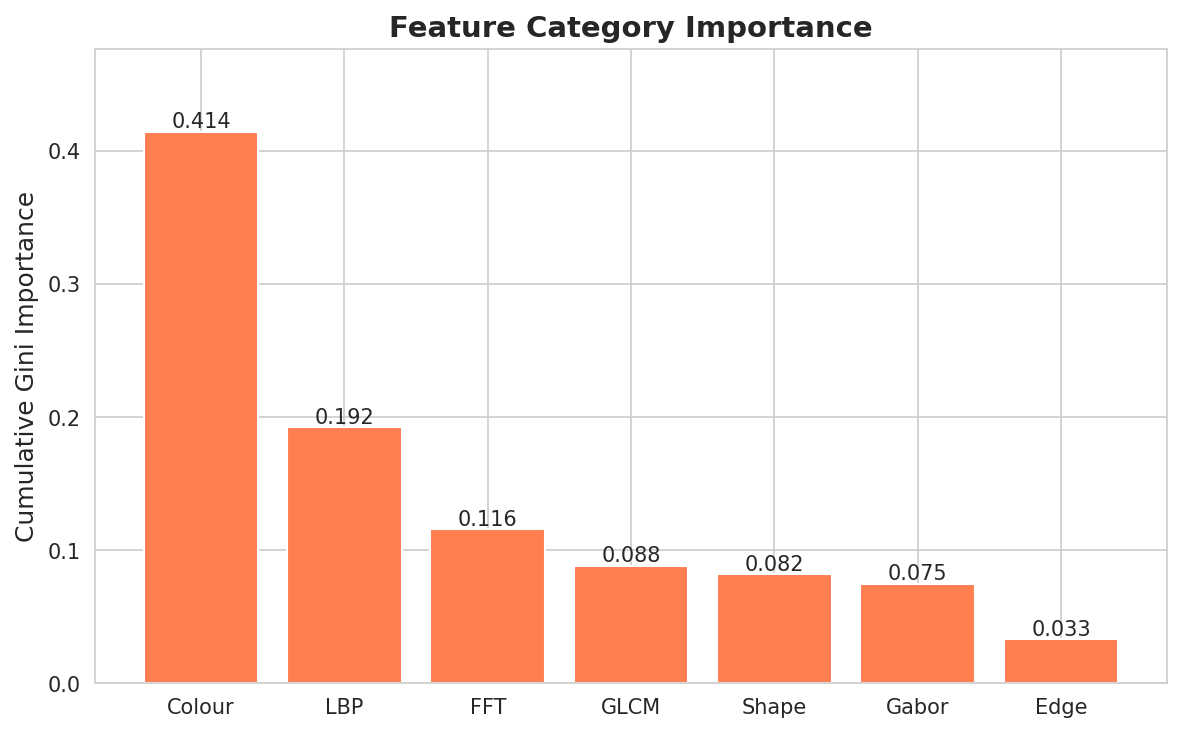
\includegraphics[width=0.9\textwidth]{category_importance.png}
            \centerline{\footnotesize Cumulative Gini importance}
        \end{column}
    \end{columns}
\end{frame}

\begin{frame}
    \frametitle{CNN Feature Extraction}
    \footnotesize
    
    \begin{columns}[T]
        \begin{column}{0.5\textwidth}
            \textbf{Transfer Learning with ResNet18}
            \vspace{0.2em}
            \begin{itemize}
                \footnotesize
                \setlength{\itemsep}{2pt}
                \item Pre-trained on ImageNet (1.2M images)
                \item Remove final FC layer
                \item Extract 512-dim embedding
                \item Inference mode (no gradients)
            \end{itemize}
            \vspace{0.3em}
            \textbf{Preprocessing}
            \begin{itemize}
                \footnotesize
                \setlength{\itemsep}{2pt}
                \item Resize to 224$\times$224
                \item ImageNet normalization
                \item $\mu = [0.485, 0.456, 0.406]$
                \item $\sigma = [0.229, 0.224, 0.225]$
            \end{itemize}
        \end{column}
        
        \begin{column}{0.45\textwidth}
            \begin{tcolorbox}[colback=ugmLightGrey,colframe=ugmBlue,title={\footnotesize Feature Representations}]
                \footnotesize
                \begin{enumerate}
                    \setlength{\itemsep}{1pt}
                    \item \textbf{Handcrafted} (155 dims)
                    \item \textbf{CNN} (512 dims)
                    \item \textbf{Hybrid (full)} (667 dims)
                    \item \textbf{Hybrid (sel.)} (200 dims, MI)
                \end{enumerate}
            \end{tcolorbox}
            \vspace{0.2em}
            \footnotesize
            All features Z-score normalized before classification.
        \end{column}
    \end{columns}
\end{frame}

\begin{frame}
    \frametitle{Classification Algorithms}
    \footnotesize
    
    \begin{columns}[T]
        \begin{column}{0.48\textwidth}
            \begin{table}
                \centering
                \footnotesize
                \begin{tabular}{ll}
                    \toprule
                    \textbf{Classifier} & \textbf{Hyperparameters} \\
                    \midrule
                    SVM (RBF) & $C=10$, $\gamma=$scale \\
                    Random Forest & 200 trees, depth=10 \\
                    XGBoost & 200 trees, depth=6 \\
                    Logistic Reg. & $C=1.0$, max iter=5000 \\
                    \bottomrule
                \end{tabular}
            \end{table}
        \end{column}
        
        \begin{column}{0.48\textwidth}
            \begin{itemize}
                \footnotesize
                \setlength{\itemsep}{2pt}
                \item 5-fold stratified CV on training set
                \item Fixed hyperparameters across all sets
                \item Independent test set evaluation
            \end{itemize}
        \end{column}
    \end{columns}
\end{frame}

% ----- SECTION: RESULTS -----
\section{Results}

\begin{frame}
    \frametitle{Classification Results}
    \footnotesize
    
    \begin{columns}[T]
        \begin{column}{0.62\textwidth}
            \begin{table}
                \centering
                \tiny
                \begin{tabular}{@{}p{1.8cm}p{1.5cm}cccc@{}}
                    \toprule
                    \textbf{Feature Set} & \textbf{Classifier} & \textbf{Acc.} & \textbf{F1} & \textbf{Test AUC} & \textbf{CV AUC} \\
                    \midrule
                    CNN (ResNet18) & SVM (RBF) & \textbf{0.855} & \textbf{0.853} & \textbf{0.949} & 0.891 \\
                    Hybrid (full) & SVM (RBF) & 0.826 & 0.825 & 0.928 & 0.915 \\
                    Hybrid (sel.) & SVM (RBF) & 0.841 & 0.840 & 0.923 & 0.916 \\
                    CNN (ResNet18) & Random Forest & 0.812 & 0.806 & 0.911 & 0.821 \\
                    CNN (ResNet18) & Logistic Reg. & 0.826 & 0.823 & 0.887 & 0.847 \\
                    Handcrafted & XGBoost & 0.754 & 0.752 & 0.840 & 0.768 \\
                    \bottomrule
                \end{tabular}
            \end{table}
        \end{column}
        
        \begin{column}{0.35\textwidth}
            \textbf{Key Findings}
            \begin{itemize}
                \footnotesize
                \setlength{\itemsep}{1pt}
                \item CNN-only dominates all baselines
                \item AUC = 0.949 (near-perfect)
                \item Hybrid competitive but not superior
                \item Handcrafted lags significantly
            \end{itemize}
        \end{column}
    \end{columns}
    
    \vspace{0.3em}
    \centerline{\alert{Best:} CNN-only + SVM (RBF) $\rightarrow$ \textbf{85.5\% accuracy, AUC = 0.949}}
\end{frame}

\begin{frame}
    \frametitle{ROC Curves}
    \footnotesize
    
    \begin{columns}[T]
        \begin{column}{0.55\textwidth}
            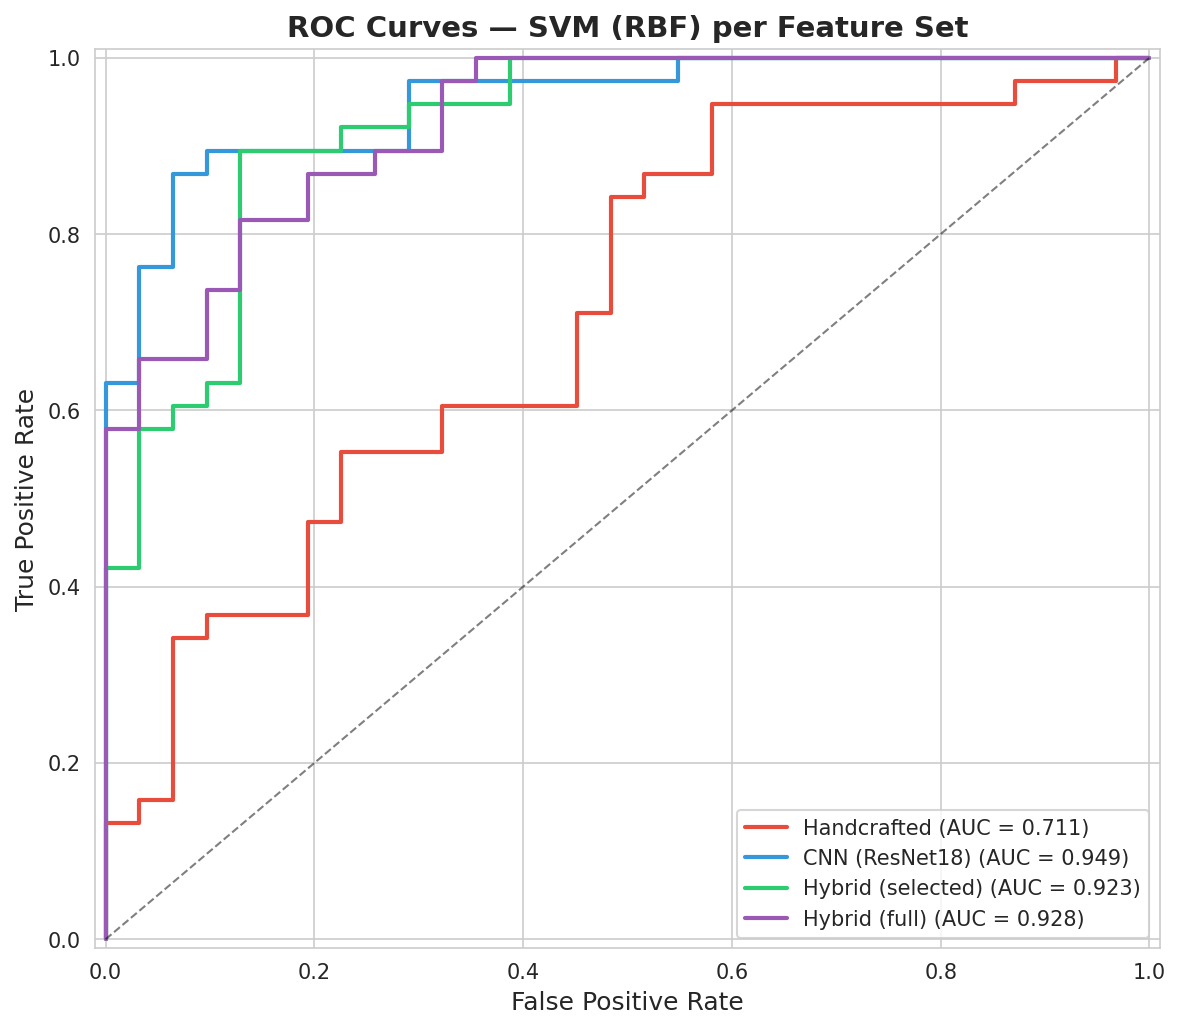
\includegraphics[width=0.9\textwidth]{roc_curves.png}
            \centerline{\footnotesize ROC curves for SVM (RBF)}
        \end{column}
        
        \begin{column}{0.4\textwidth}
            \textbf{Observations}
            \begin{itemize}
                \footnotesize
                \setlength{\itemsep}{2pt}
                \item CNN-only dominates all sets
                \item AUC = 0.949 (near-perfect)
                \item Hybrid competitive but not superior
                \item Handcrafted lags significantly
            \end{itemize}
        \end{column}
    \end{columns}
\end{frame}

\begin{frame}
    \frametitle{Confusion Matrix \& Classification Report}
    \footnotesize
    
    \begin{columns}[T]
        \begin{column}{0.32\textwidth}
            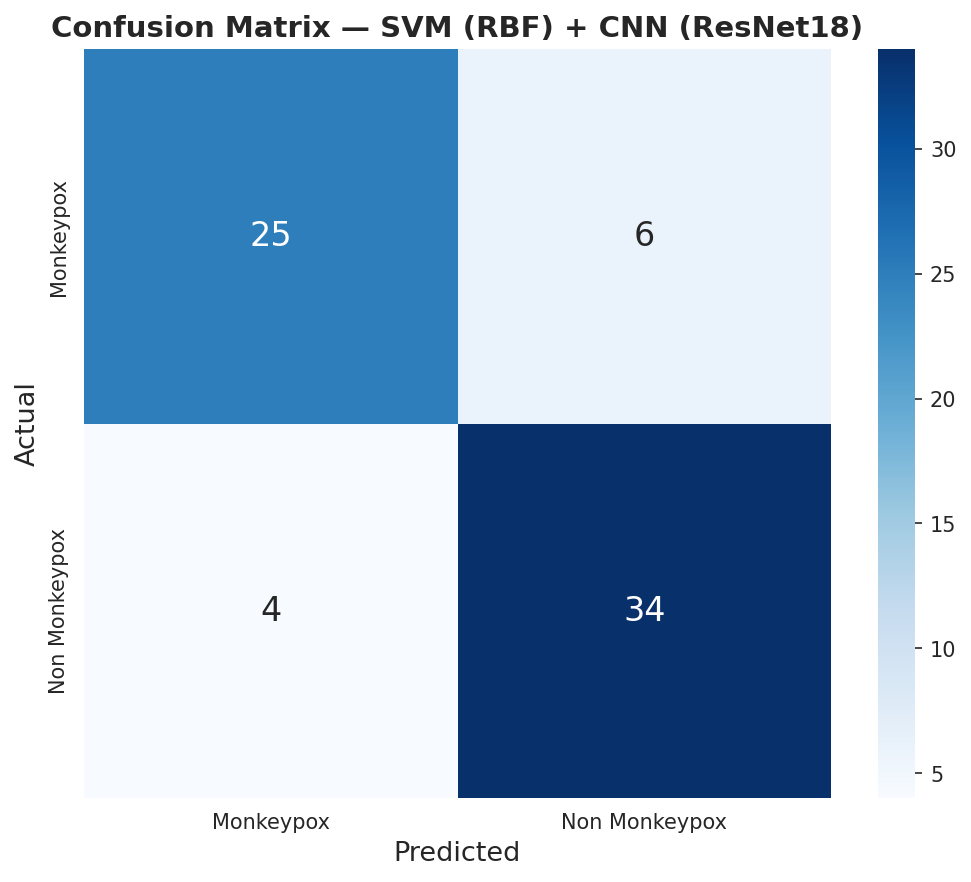
\includegraphics[width=\textwidth]{confusion_matrix.png}
            \centerline{\footnotesize Confusion matrix}
        \end{column}
        
        \begin{column}{0.63\textwidth}
            \textbf{Classification Report (SVM + CNN-only)}
            \vspace{0.2em}
            \footnotesize
            \begin{table}
                \centering
                \begin{tabular}{@{}lccc@{}}
                    \toprule
                    \textbf{Class} & \textbf{Precision} & \textbf{Recall} & \textbf{F1} \\
                    \midrule
                    Monkeypox & 0.86 & 0.81 & 0.83 \\
                    Non-Monkeypox & 0.85 & 0.89 & 0.87 \\
                    \midrule
                    \textbf{Macro Avg} & 0.86 & 0.85 & 0.85 \\
                    \bottomrule
                \end{tabular}
            \end{table}
            \vspace{0.2em}
            \begin{itemize}
                \footnotesize
                \setlength{\itemsep}{1pt}
                \item 81\% MPX recall, 89\% non-MPX recall
                \item Balanced false positives / false negatives
                \item Overall macro F1 = 0.85
            \end{itemize}
        \end{column}
    \end{columns}
\end{frame}

\begin{frame}
    \frametitle{Feature Space Visualization}
    \footnotesize
    
    \begin{columns}[T]
        \begin{column}{0.48\textwidth}
            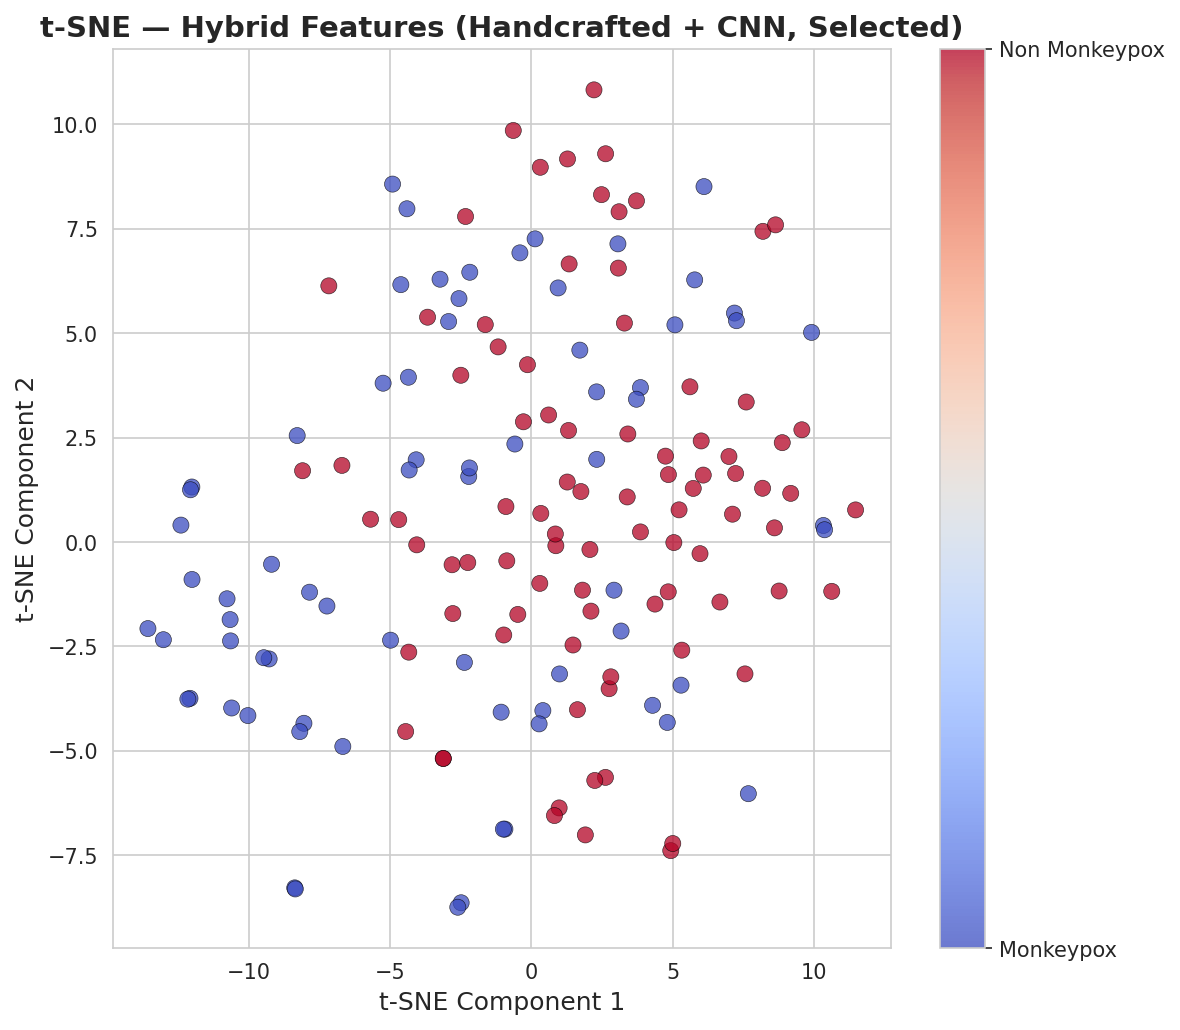
\includegraphics[width=0.85\textwidth]{tsne_hybrid.png}
            \centerline{\footnotesize t-SNE (hybrid selected)}
        \end{column}
        
        \begin{column}{0.48\textwidth}
            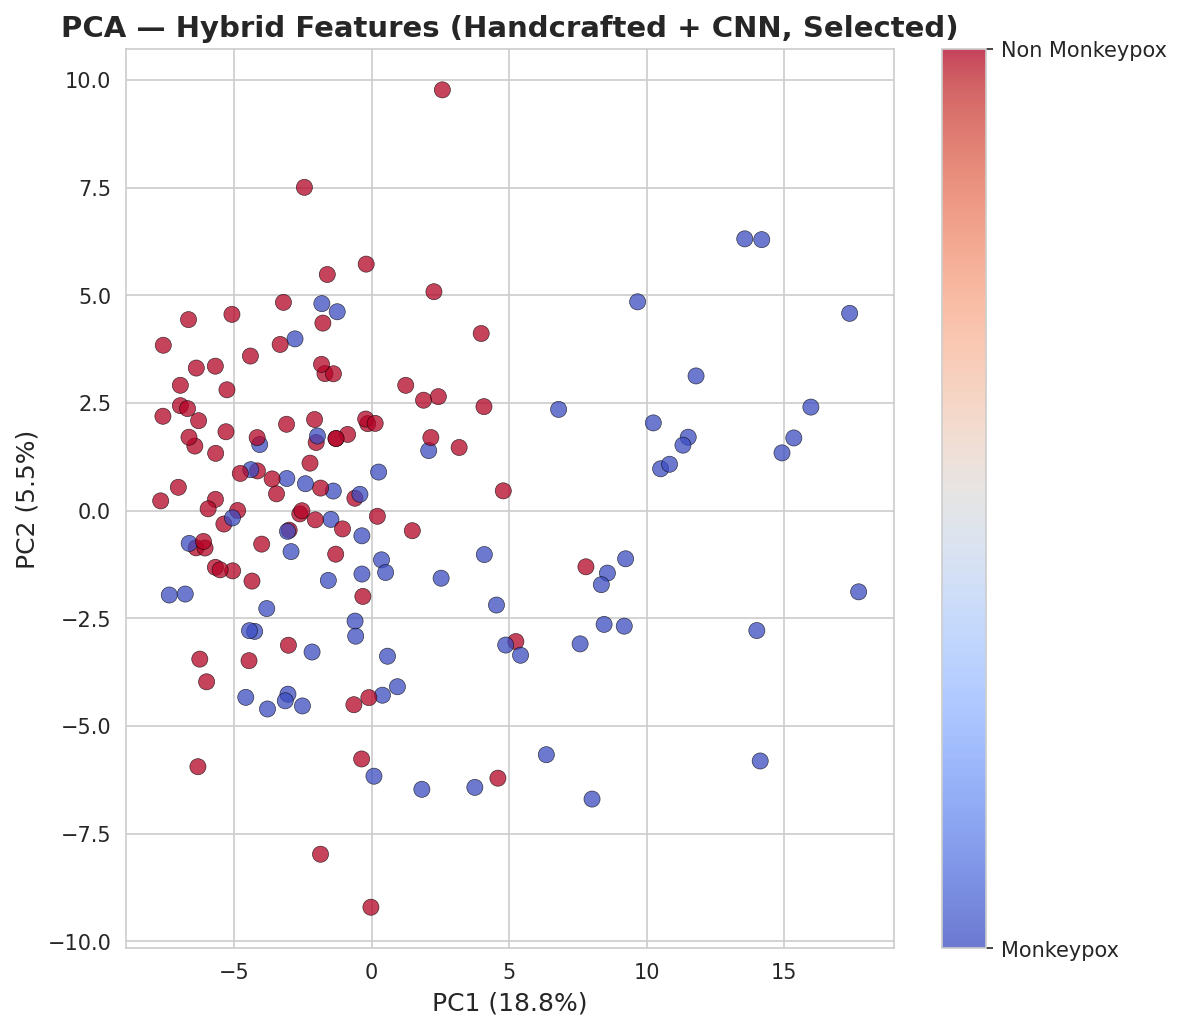
\includegraphics[width=0.85\textwidth]{pca_hybrid.png}
            \centerline{\footnotesize PCA (hybrid selected)}
        \end{column}
    \end{columns}
    
    \vspace{0.2em}
    \centerline{\footnotesize Moderate separability; overlap consistent with challenging visual diagnosis}
\end{frame}

\begin{frame}
    \frametitle{Feature Importance Analysis}
    \footnotesize
    
    \begin{columns}[T]
        \begin{column}{0.48\textwidth}
            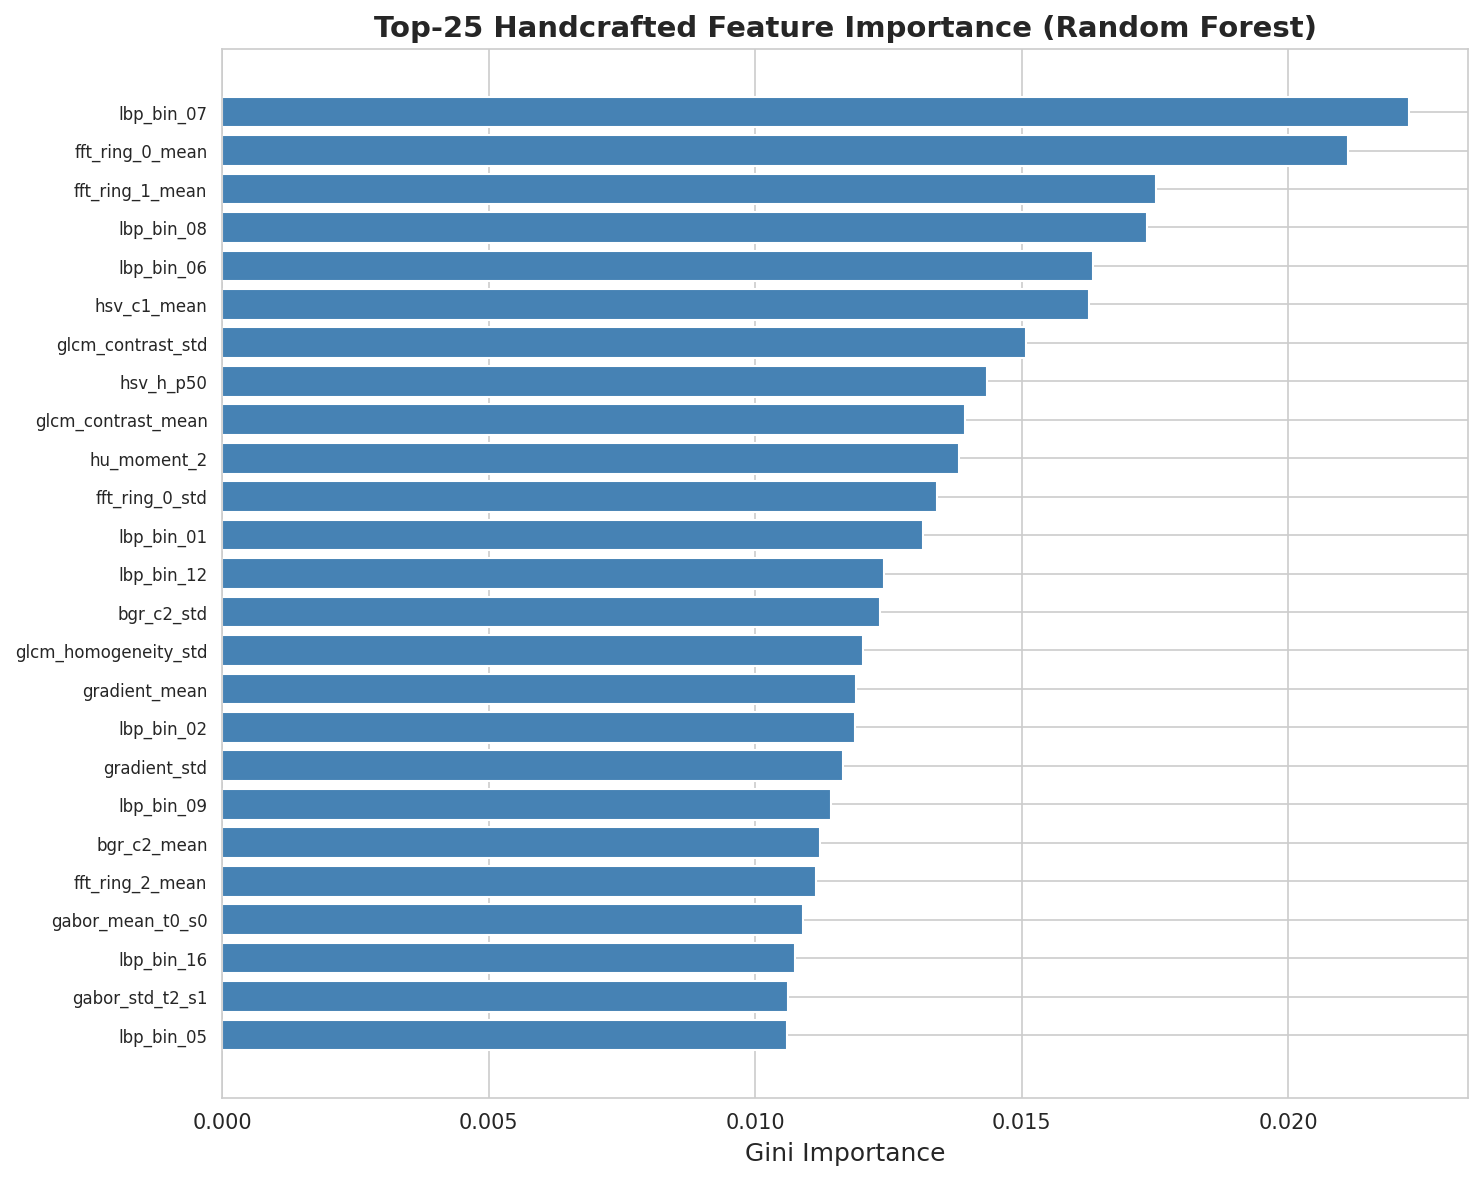
\includegraphics[width=0.85\textwidth]{feature_importance.png}
            \centerline{\footnotesize Top-25 handcrafted features (RF)}
        \end{column}
        
        \begin{column}{0.48\textwidth}
            \textbf{Key Findings}
            \begin{itemize}
                \footnotesize
                \setlength{\itemsep}{1pt}
                \item \textbf{Color features} most important (HSV/LAB)
                \item \textbf{GLCM texture} second most discriminative
                \item Gabor and edge features also contribute
                \item Aligns with dermatology:
                \begin{itemize}
                    \footnotesize
                    \setlength{\itemsep}{1pt}
                    \item MPX: red-purple hues
                    \item Umbilicated vesicle textures
                \end{itemize}
            \end{itemize}
        \end{column}
    \end{columns}
\end{frame}

% ----- SECTION: DISCUSSION -----
\section{Discussion}

\begin{frame}
    \frametitle{Discussion}
    \footnotesize
    
    \begin{columns}[T]
        \begin{column}{0.48\textwidth}
            \begin{block}{\footnotesize CNN Features}
                \footnotesize
                \begin{itemize}
                    \setlength{\itemsep}{1pt}
                    \item ResNet18 highly effective \textbf{without fine-tuning}
                    \item Captures shape, color, texture patterns
                    \item Best: AUC = 0.949
                \end{itemize}
            \end{block}
            
            \begin{exampleblock}{\footnotesize Handcrafted Features}
                \footnotesize
                \begin{itemize}
                    \setlength{\itemsep}{1pt}
                    \item Moderate (best AUC = 0.840)
                    \item Color and GLCM most important
                    \item Interpretable and lightweight
                \end{itemize}
            \end{exampleblock}
        \end{column}
        
        \begin{column}{0.48\textwidth}
            \begin{alertblock}{\footnotesize Hybrid Approach}
                \footnotesize
                \begin{itemize}
                    \setlength{\itemsep}{1pt}
                    \item Did \textbf{not} surpass CNN-only baseline
                    \item 228 samples: 667 dims overfits
                    \item Selection (200 dims) helps but still below CNN
                    \item May win with larger dataset
                \end{itemize}
            \end{alertblock}
            
            \begin{tcolorbox}[colback=ugmLightGrey,colframe=ugmBlue,title={\footnotesize Classifier Choice}]
                \footnotesize
                SVM (RBF) consistently best across all feature sets -- non-linear boundary in high-dim space.
            \end{tcolorbox}
        \end{column}
    \end{columns}
\end{frame}

% ----- SECTION: CONCLUSION -----
\section{Conclusion}

\begin{frame}
    \frametitle{Conclusion \& Future Work}
    \footnotesize
    
    \begin{columns}[T]
        \begin{column}{0.48\textwidth}
            \textbf{Summary}
            \begin{enumerate}
                \footnotesize
                \setlength{\itemsep}{1pt}
                \item LAB-based lesion segmentation
                \item 7-category handcrafted features (155 dims)
                \item ResNet18 CNN embeddings (512 dims)
                \item Systematic comparison across 4 classifiers
                \item \textbf{Best: 85.5\% accuracy, AUC = 0.949}
            \end{enumerate}
        \end{column}
        
        \begin{column}{0.48\textwidth}
            \textbf{Future Work}
            \begin{itemize}
                \footnotesize
                \setlength{\itemsep}{1pt}
                \item Larger multi-center dataset
                \item Attention mechanisms for highlighting
                \item Lightweight mobile deployment
                \item Multi-CNN ensemble methods
            \end{itemize}
        \end{column}
    \end{columns}
\end{frame}

% ----- REFERENCES -----
\section*{References}

\begin{frame}
    \frametitle{References}
    \scriptsize
    \begin{thebibliography}{9}
        \setlength{\itemsep}{1pt}
        \bibitem{kaggle} N.~A.~Mahmud et al., ``Monkeypox Skin Lesion Dataset,'' Kaggle, 2022.
        \bibitem{codella} N.~Codella et al., ``Skin lesion analysis toward melanoma detection 2018,'' \textit{IEEE Trans. Med. Imag.}, 2018.
        \bibitem{haralick} R.~M.~Haralick et al., ``Textural features for image classification,'' \textit{IEEE Trans. SMC}, 1973.
        \bibitem{ojala} T.~Ojala et al., ``Multiresolution gray-scale and rotation invariant texture classification with LBP,'' \textit{IEEE TPAMI}, 2002.
        \bibitem{he} K.~He et al., ``Deep residual learning for image recognition,'' \textit{Proc. CVPR}, 2016.
        \bibitem{ozkan} I.~A.~Ozkan and A.~Dana, ``Deep learning-based feature extraction for melanoma,'' \textit{Biomed. Signal Proc.}, 2021.
    \end{thebibliography}
\end{frame}

% ----- THANK YOU -----
\begin{frame}[plain]
    \vspace{3cm}
    \begin{center}
        \Huge\textbf{Thank You}
        \vspace{1cm}
        
        \Large Questions?
        \vspace{1.5cm}
        
        \normalsize
        \textbf{Yusuf Imantaka Bastari} \& \textbf{Aufa Sultan Syach Majid Putra Yuliyanto}\\
        Department of Computer Science and Electronics\\
        Universitas Gadjah Mada, Yogyakarta, Indonesia\\
        yusufimantakabastari@mail.ugm.ac.id
    \end{center}
\end{frame}

\end{document}
